\documentclass[11pt]{article}

\usepackage[letterpaper,margin=0.82in]{geometry}
\usepackage[T1]{fontenc}
\usepackage[utf8]{inputenc}
\usepackage{lmodern}
\usepackage{microtype}
\usepackage{graphicx}
\usepackage{booktabs}
\usepackage{tabularx}
\usepackage{longtable}
\usepackage{array}
\usepackage{amsmath,amssymb,mathtools,bm}
\usepackage{xcolor}
\usepackage{enumitem}
\usepackage{hyperref}
\usepackage{cleveref}
\usepackage[most]{tcolorbox}
\usepackage{fancyhdr}
\usepackage{titlesec}
\usepackage{url}
\usepackage{float}
\usepackage{listings}
\usepackage{tikz}
\usetikzlibrary{arrows.meta,positioning,fit,calc,shapes.geometric,backgrounds}

\definecolor{navy}{HTML}{17365D}
\definecolor{bluebox}{HTML}{EAF2FF}
\definecolor{orangebox}{HTML}{FFF0E2}
\definecolor{greenbox}{HTML}{EAF8EE}
\definecolor{purplebox}{HTML}{F0ECFF}
\definecolor{graybox}{HTML}{F5F6F7}
\definecolor{darkgray}{HTML}{374151}
\definecolor{accent}{HTML}{E97800}
\definecolor{green}{HTML}{16843D}
\definecolor{red}{HTML}{B42318}
\definecolor{codegreen}{HTML}{1A7F37}

\hypersetup{
  colorlinks=true,
  hypertexnames=false,
  linkcolor=navy,
  citecolor=navy,
  urlcolor=navy,
  pdftitle={Generalized Adaptive Physics Embedding Architecture Plan},
  pdfauthor={World Model Robotics Design Study}
}

\pagestyle{fancy}
\fancyhf{}
\lhead{Generalized Adaptive Physics Embedding}
\rhead{Variable Metadata Teacher + Causal Student}
\cfoot{\thepage}
\setlength{\headheight}{14pt}

\titleformat{\section}{\Large\bfseries\color{navy}}{\thesection}{0.7em}{}
\titleformat{\subsection}{\large\bfseries\color{darkgray}}{\thesubsection}{0.6em}{}
\titleformat{\subsubsection}{\normalsize\bfseries\color{darkgray}}{\thesubsubsection}{0.5em}{}

\setlist[itemize]{leftmargin=1.35em,itemsep=0.22em,topsep=0.35em}
\setlist[enumerate]{leftmargin=1.55em,itemsep=0.25em,topsep=0.35em}
\renewcommand{\arraystretch}{1.16}

\newcolumntype{Y}{>{\raggedright\arraybackslash}X}
\newcolumntype{L}[1]{>{\raggedright\arraybackslash}p{#1}}
\newcolumntype{C}[1]{>{\centering\arraybackslash}p{#1}}

\newtcolorbox{decisionbox}[1][]{
  enhanced,colback=greenbox,colframe=green,boxrule=0.9pt,arc=2mm,
  left=2mm,right=2mm,top=1.5mm,bottom=1.5mm,
  title=Recommended decision,fonttitle=\bfseries,#1
}

\newtcolorbox{warningbox}[1][]{
  enhanced,colback=orangebox,colframe=accent,boxrule=0.9pt,arc=2mm,
  left=2mm,right=2mm,top=1.5mm,bottom=1.5mm,
  title=Important boundary,fonttitle=\bfseries,#1
}

\newtcolorbox{gatebox}[1][]{
  enhanced,colback=bluebox,colframe=navy,boxrule=0.75pt,arc=1.5mm,
  left=2mm,right=2mm,top=1.5mm,bottom=1.5mm,
  title=Go/no-go rule,fonttitle=\bfseries,#1
}

\newtcolorbox{plainbox}[1][]{
  enhanced,colback=graybox,colframe=darkgray,boxrule=0.6pt,arc=1.5mm,
  left=2mm,right=2mm,top=1.5mm,bottom=1.5mm,#1
}

\lstdefinestyle{pythonstyle}{
  language=Python,
  basicstyle=\ttfamily\footnotesize,
  keywordstyle=\color{navy}\bfseries,
  commentstyle=\color{codegreen},
  stringstyle=\color{accent},
  showstringspaces=false,
  breaklines=true,
  frame=single,
  rulecolor=\color{gray!45},
  backgroundcolor=\color{gray!4},
  columns=fullflexible,
  keepspaces=true
}

\newcommand{\bvec}{\bm b}
\newcommand{\zvec}{\bm z}
\newcommand{\avec}{\bm a}
\newcommand{\svec}{\bm s}
\newcommand{\R}{\mathbb R}
\newcommand{\E}{\mathbb E}
\newcommand{\sg}{\operatorname{sg}}
\newcommand{\pool}{\operatorname{Pool}}
\newcommand{\FM}{\mathcal L_{\mathrm{FM}}}
\newcommand{\meta}{\mathcal M}

\begin{document}
\pagenumbering{gobble}

\begin{titlepage}
\centering
\vspace*{0.50in}
{\Huge\bfseries\color{navy} Generalized Adaptive Physics\\[0.10in]
Embedding Architecture Plan\par}
\vspace{0.24in}
{\Large Variable-schema simulation supervision, causal video inference,\\
and compact Wan conditioning\par}
\vspace{0.42in}

\begin{tcolorbox}[width=0.89\textwidth,colback=bluebox,colframe=navy,boxrule=1pt,arc=2mm]
\centering
\large
Replace the fixed projectile-specific parameter vector with a
\textbf{variable-length set of typed metadata records}.  A simulation-only
teacher compresses any record set into one fixed-size dynamics belief.  A
causal student infers the same belief from ordered Wan-VAE latents, executed
actions, and robot state.  The belief is projected into a fixed set of physics
tokens and injected through a small number of zero-gated Wan adapters.
\end{tcolorbox}

\vfill
{\large Modified architecture and executable training plan\par}
\vspace{0.12in}
{\large July 2026\par}
\vspace{0.35in}
{\small Prepared for the World Model Robotics project\par}
\end{titlepage}

\clearpage
\pagenumbering{roman}
\tableofcontents
\clearpage
\pagenumbering{arabic}

\section{Executive decision}

\begin{decisionbox}
Build the first generalized system with exactly five core modules:
\begin{enumerate}
  \item a frozen Wan VAE and versioned latent cache;
  \item a permutation-invariant metadata teacher that accepts a variable number
  of typed simulator records and outputs a fixed 64-dimensional belief;
  \item a temporally ordered student that infers the same 64-dimensional belief
  from a sliding window of VAE latents, actions, and robot state;
  \item one shared projector from the compact belief to eight 256-dimensional
  physics tokens;
  \item four small, zero-gated physics cross-attention adapters distributed
  through the Wan DiT.
\end{enumerate}
Use sliding-window recomputation as the first adaptive mechanism.  Do not put
probabilistic sampling, recurrent filtering, EMA self-distillation, a latent
predictor, gradient refinement, physics LoRA, or explicit object/relation token
graphs in version 1.
\end{decisionbox}

The core interface is
\begin{equation}
  \underbrace{\meta_t=\{m_{t,j}\}_{j=1}^{n_t}}_{
  \substack{\text{variable number of}\\\text{simulation records}}}
  \xrightarrow{\;T_\psi\;}
  \underbrace{\bvec_t^T\in\R^{d_b}}_{\text{fixed teacher belief}},
  \qquad
  \underbrace{h_t=(Z_{t-W+1:t},a,s)}_{\text{deployment history}}
  \xrightarrow{\;S_\phi\;}
  \underbrace{\bvec_t^S\in\R^{d_b}}_{\text{fixed student belief}},
  \label{eq:two-paths}
\end{equation}
with
\begin{equation}
  C_t^{\mathrm{phys}}=P_\eta(\bvec_t)\in\R^{K\times d_{\mathrm{phys}}}.
  \label{eq:projector}
\end{equation}
The record count $n_t$, property names, and available subsets may change across
tasks; $d_b$, $K$, and the Wan interface do not.

\begin{plainbox}[title=Plain-language summary]
The simulator teacher is allowed to read the configuration file.  The real
robot student is not.  Both must produce the same compact ``how this scene
behaves'' code.  Wan receives that code in a fixed format.  When a new
interaction is observed, the student reruns on the latest history window and
produces a revised code.
\end{plainbox}

\section{What changes relative to the current design}

\begin{figure}[H]
\centering
\includegraphics[width=0.98\textwidth]{current_architecture.png}
\caption{Current projectile-specific system.  The fixed Wan conditioning
interface is useful; the fixed 14-dimensional semantic schema and its
privileged availability at deployment are the specialized parts.}
\label{fig:current}
\end{figure}

The proposed architecture retains the final conditioning interface but changes
both sources of physics information:
\begin{itemize}
  \item the simulation branch no longer assumes one vector with one fixed
  dimension and ordering;
  \item the deployment branch infers the code from ordered intervention-response
  history instead of requiring metadata.
\end{itemize}

\begin{table}[H]
\centering
\small
\caption{Essential components versus deferred or removed components.}
\begin{tabularx}{\textwidth}{L{0.22\textwidth} C{0.12\textwidth} Y}
\toprule
Component & Decision & Reason \\
\midrule
Frozen Wan VAE & Keep & Shared latent substrate for student inference and Wan generation; enables caching. \\
Temporal positions and action alignment & Keep & Physics identification requires knowing which action caused which response. \\
Variable-record metadata teacher & Keep & Directly addresses variable parameter count and heterogeneous task schemas. \\
Compact fixed belief & Keep & Stable teacher-student target and stable Wan interface. \\
Shared mean-only projector & Keep & Prevents teacher/student interface drift and avoids uncertainty as a side channel. \\
Four separate physics adapters & Keep & Clean ablation and low trainable footprint; four is the initial minimum, not a permanent limit. \\
Explicit $\Delta Z$ branch & Optional & Adds no new information; concatenate $[Z;\Delta Z]$ only if it improves optimization. \\
Probabilistic student & Defer & Deterministic inference must first establish that the core code is identifiable and useful. \\
Multiple-window fusion & Remove & Overlapping windows are correlated and can create false confidence. \\
Recurrent belief updater & Defer & Sliding-window recomputation is already adaptive and easier to validate. \\
Latent predictor / EMA / gradient refinement & Defer & Needed only for unlabeled real adaptation or test-time optimization, not the core simulation-to-student test. \\
Physics LoRA & Remove initially & A second Wan-side adaptation path makes attribution and debugging harder. \\
Object/relation token graph & Remove initially & Variable object and pair counts create avoidable complexity; test a global fixed belief first. \\
\bottomrule
\end{tabularx}
\end{table}

\section{End-to-end architecture}

\begin{figure}[H]
\centering
\resizebox{\textwidth}{!}{%
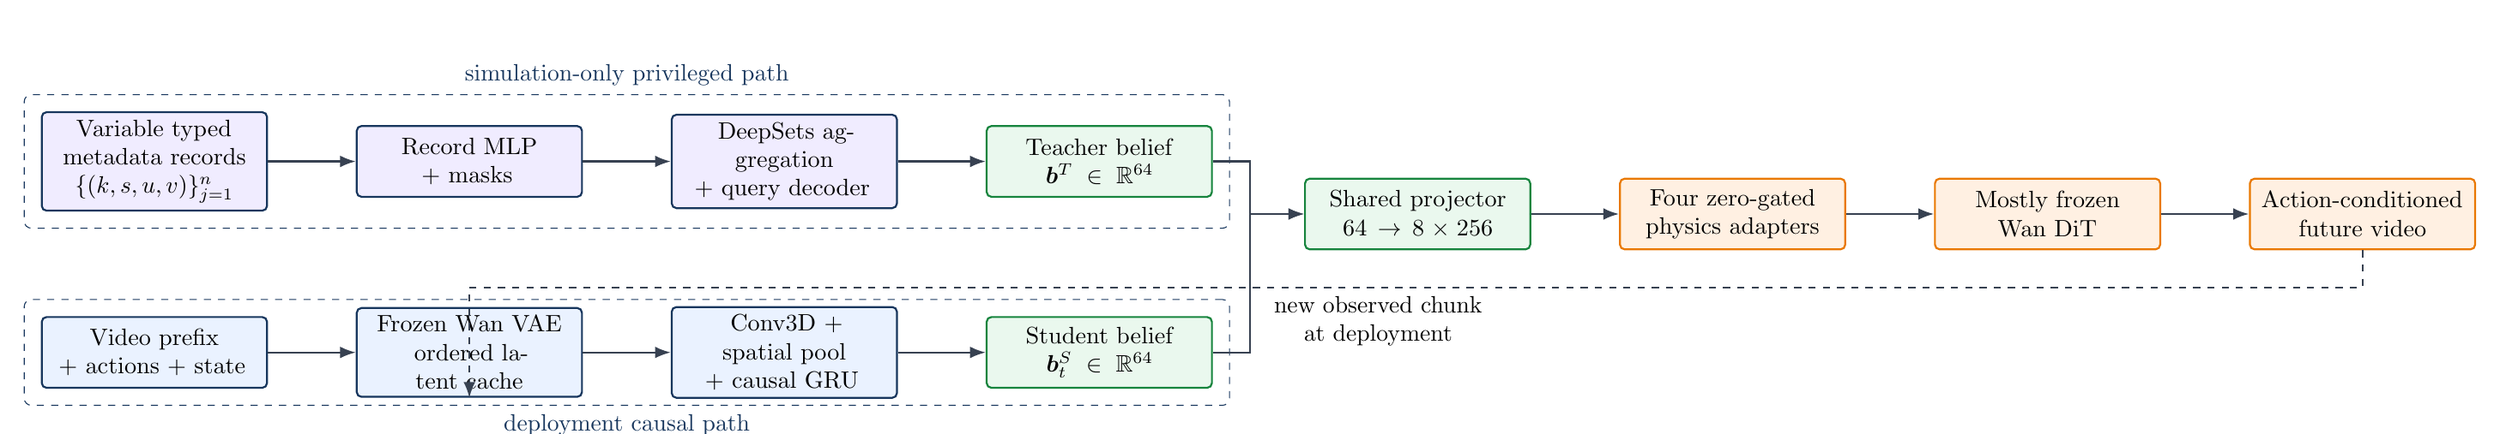
\begin{tikzpicture}[
  node distance=1.0cm and 1.3cm,
  block/.style={draw,rounded corners=2pt,minimum height=1.05cm,align=center,text width=3.1cm,thick},
  sim/.style={block,fill=purplebox,draw=navy},
  obs/.style={block,fill=bluebox,draw=navy},
  core/.style={block,fill=greenbox,draw=green},
  wan/.style={block,fill=orangebox,draw=accent},
  arr/.style={-Latex,thick,draw=darkgray}
]
  \node[sim] (meta) {Variable typed metadata records\\$\{(k,s,u,v)\}_{j=1}^{n}$};
  \node[sim,right=of meta] (rec) {Record MLP\\+ masks};
  \node[sim,right=of rec] (set) {DeepSets aggregation\\+ query decoder};
  \node[core,right=of set] (bt) {Teacher belief\\$\bvec^T\in\R^{64}$};

  \node[obs,below=1.55cm of meta] (video) {Video prefix\\+ actions + state};
  \node[obs,right=of video] (vae) {Frozen Wan VAE\\ordered latent cache};
  \node[obs,right=of vae] (student) {Conv3D + spatial pool\\+ causal GRU};
  \node[core,right=of student] (bs) {Student belief\\$\bvec_t^S\in\R^{64}$};

  \node[core,right=1.35cm of bt,yshift=-0.78cm] (proj) {Shared projector\\$64\rightarrow 8\times256$};
  \node[wan,right=of proj] (adapt) {Four zero-gated\\physics adapters};
  \node[wan,right=of adapt] (dit) {Mostly frozen\\Wan DiT};
  \node[wan,right=of dit] (future) {Action-conditioned\\future video};

  \draw[arr] (meta) -- (rec);
  \draw[arr] (rec) -- (set);
  \draw[arr] (set) -- (bt);
  \draw[arr] (video) -- (vae);
  \draw[arr] (vae) -- (student);
  \draw[arr] (student) -- (bs);
  \draw[arr] (bt.east) -- ++(0.55,0) |- (proj.west);
  \draw[arr] (bs.east) -- ++(0.55,0) |- (proj.west);
  \draw[arr] (proj) -- (adapt);
  \draw[arr] (adapt) -- (dit);
  \draw[arr] (dit) -- (future);
  \draw[arr,dashed] (future.south) -- ++(0,-0.55) -| node[pos=0.26,below,align=center]{new observed chunk\\at deployment} (vae.south);

  \begin{scope}[on background layer]
    \node[draw=navy,dashed,rounded corners=3pt,fit=(meta)(bt),inner sep=7pt,label={[navy]above:simulation-only privileged path}] {};
    \node[draw=navy,dashed,rounded corners=3pt,fit=(video)(bs),inner sep=7pt,label={[navy]below:deployment causal path}] {};
  \end{scope}
\end{tikzpicture}}
\caption{Recommended generalized architecture.  Input cardinality varies only
inside the metadata teacher and the observed history.  The belief and Wan
conditioning interfaces remain fixed.}
\label{fig:architecture}
\end{figure}

\subsection{Core invariants}

The design should preserve the following invariants throughout implementation:
\begin{enumerate}
  \item \textbf{Causal student:} $\bvec_t^S$ uses only observations and executed
  controls at or before $t$.
  \item \textbf{Dynamics-oriented bottleneck:} the belief is small enough that
  it cannot simply copy all spatial VAE content.
  \item \textbf{Teacher/student symmetry:} both paths terminate at the same
  belief shape and use the same projector.
  \item \textbf{Permutation-invariant metadata input:} reordering metadata
  records leaves the teacher belief unchanged.
  \item \textbf{Fixed Wan interface:} changing the task schema never changes the
  number or width of Wan physics tokens.
  \item \textbf{Counterfactual dependence:} Wan must distinguish correct from
  wrong physics while all other inputs are held fixed.
\end{enumerate}

\section{Module A: variable-length metadata teacher}

\subsection{Record schema}

Represent simulator metadata as a set
\begin{equation}
  \meta_t=\{m_{t,j}\}_{j=1}^{n_t},
  \qquad
  m_{t,j}=(k_j,s_j,u_j,v_j),
  \label{eq:metadata-set}
\end{equation}
where:
\begin{itemize}
  \item $k_j$ is a property key such as \texttt{mass},
  \texttt{dynamic\_friction}, or \texttt{bending\_stiffness};
  \item $s_j$ is a canonical semantic scope such as \texttt{global},
  \texttt{primary\_object}, or
  \path{primary_object--support_surface};
  \item $u_j$ is a unit or physical-dimension descriptor;
  \item $v_j$ is the scalar value in a canonical unit system.
\end{itemize}

Use one scalar record per vector component.  For example, gravity becomes
\texttt{gravity\_x}, \texttt{gravity\_y}, and \texttt{gravity\_z}.  Require a
unique $(k,s)$ pair within one episode; if a simulator exposes repeated fields,
first canonicalize them into distinct semantic roles.

\begin{lstlisting}[style=pythonstyle,caption={Example variable-length metadata records.}]
metadata = [
    {"key": "gravity_z", "scope": "global",
     "unit": "m/s^2", "value": -9.81},
    {"key": "mass", "scope": "primary_object",
     "unit": "kg", "value": 0.20},
    {"key": "dynamic_friction",
     "scope": "primary_object--support_surface",
     "unit": "dimensionless", "value": 0.35},
    {"key": "restitution",
     "scope": "primary_object--support_surface",
     "unit": "dimensionless", "value": 0.72},
]
\end{lstlisting}

\subsection{Canonicalization and normalization}

Do not pass raw simulator body IDs such as \texttt{body\_17}.  They have no
stable visual meaning.  Begin with a small role vocabulary:
\begin{center}
\texttt{global}, \texttt{robot}, \texttt{primary\_object},
\texttt{secondary\_object}, \texttt{support\_surface}, \texttt{joint},
\texttt{material}, and canonical pair roles.
\end{center}

Convert values to canonical units where possible.  Normalize each property key
using training-set statistics:
\begin{equation}
  \widetilde v_j=\frac{g_{k_j}(v_j)-\mu_{k_j}}{\sigma_{k_j}+\epsilon},
  \label{eq:value-normalize}
\end{equation}
where $g_k$ is the identity for bounded values and a log transform for positive
quantities spanning several orders of magnitude.  Store $\mu_k$, $\sigma_k$,
and the transform in the dataset manifest.

A more portable unit representation uses a seven-dimensional SI exponent
signature together with a small unit-family embedding.  A simpler unit-ID
embedding is acceptable for the first implementation after all values have
been converted to canonical units.

\subsection{Record encoder and DeepSets aggregation}

Encode each record as
\begin{equation}
  r_j=f_{\mathrm{rec}}\!\left(
  [E_k(k_j);E_s(s_j);E_u(u_j);\widetilde v_j]
  \right)\in\R^{d_r}.
  \label{eq:record-encoder}
\end{equation}
Use $d_r=256$ and a two-layer MLP.  Aggregate a masked record set with
\begin{equation}
  q=\left[
  \frac{1}{\sqrt{n}}\sum_{j=1}^{n}\phi(r_j);
  \log(1+n)
  \right],
  \qquad
  \bvec^T=\rho(q)\in\R^{d_b}.
  \label{eq:deepsets}
\end{equation}
This is permutation invariant and linear in record count.  Use $d_b=64$ first.
A Set Transformer is a later replacement only if the DeepSets teacher fails a
measured interaction test.

Do not apply per-sample LayerNorm to the final belief.  It couples code
dimensions and makes later uncertainty modeling difficult.  Use a small output
scale, optional \texttt{tanh}, and batch-level statistics if needed.

\subsection{Metadata query decoder}

A variable-schema teacher needs a variable-schema supervision head.  Given a
query for property $(k_j,s_j,u_j)$, decode its normalized value:
\begin{equation}
  \widehat v_j=D_\omega\!\left(
  \bvec^T,E_k(k_j),E_s(s_j),E_u(u_j)
  \right).
  \label{eq:query-decoder}
\end{equation}
The teacher metadata loss is
\begin{equation}
  \mathcal L_{\mathrm{meta}}
  =\frac{1}{n}\sum_{j=1}^{n}
  \left\lVert\widehat v_j-\widetilde v_j\right\rVert_2^2.
  \label{eq:meta-loss}
\end{equation}
The decoder replaces fixed 14-dimensional reconstruction.  It evaluates only
records that exist in the episode, so missing parameters require no padding in
the semantic target.

\begin{warningbox}
Variable input length does not mean unlimited zero-shot semantics.  Adding a
new property key leaves the belief and Wan dimensions unchanged, but the new
key embedding and decoder behavior still require training or fine-tuning.
A text encoder over property names is a possible later extension, not a reason
to skip a controlled key registry in the first system.
\end{warningbox}

\section{Module B: causal student from Wan-VAE history}

\subsection{Inputs}

At deployment, the student receives only
\begin{equation}
  h_t=\left(
  Z_{t-W+1:t},
  a_{t-W+1:t-1},
  s_{t-W+1:t}
  \right),
  \label{eq:student-history}
\end{equation}
where $Z$ is the frozen Wan-VAE latent sequence, $a$ contains executed actions,
and $s$ contains robot state and any deployment-available sensors.  A fixed
window $W$ is used in version 1.  Do not fuse several overlapping windows.

Actions are not optional.  The same displacement can result from a weak action
on a light object or a strong action on a heavy object.  Physics identification
requires the intervention and the response.

\subsection{Visual evidence encoder}

Optionally concatenate temporal differences:
\begin{equation}
  X=[Z;\Delta Z],
  \qquad
  \Delta Z_t=Z_t-Z_{t-1}.
\end{equation}
Mask the causal-VAE first-chunk boundary where this difference is not
comparable.  Since $\Delta Z$ is deterministic from $Z$, treat it as an
optimization ablation rather than an essential source.

Use a spatial Conv3D stem with temporal kernel one:
\begin{equation}
  F=\operatorname{Conv3D}(X)
  \in\R^{B\times d_v\times T_z\times H'\times W'}.
\end{equation}
Add factorized time and spatial positions:
\begin{equation}
  \widetilde F_{t,h,w}=F_{t,h,w}+p_t+p_h+p_w.
\end{equation}
Pool each latent time bin into one visual evidence vector with a learned query:
\begin{equation}
  e_t^{\mathrm{vis}}
  =\operatorname{AttnPool}_{h,w}(\widetilde F_{t,h,w})
  \in\R^{256}.
  \label{eq:spatial-pool}
\end{equation}
This is far smaller than eight learned queries per time bin and is sufficient
for the first test.

\subsection{Action and robot-state alignment}

Map high-rate controls to the same VAE latent bins.  Let $\mathcal I(t)$ be the
control samples associated with latent bin $t$.  Use
\begin{equation}
  e_t^{\mathrm{ctrl}}
  =E_{\mathrm{ctrl}}\!\left(
  \{(a_\tau,s_\tau):\tau\in\mathcal I(t)\}
  \right).
  \label{eq:control-encoder}
\end{equation}
Use an MLP when there is one control sample per latent bin; use a small GRU or
temporal convolution when several samples must be aggregated.  Mean pooling is
not sufficient because it destroys impulse timing.

\subsection{Temporal inference and belief output}

Fuse visual and control evidence:
\begin{equation}
  x_t=W_x[e_t^{\mathrm{vis}};e_t^{\mathrm{ctrl}}]+p_t.
\end{equation}
Run a two-layer causal GRU:
\begin{equation}
  h_t^{\mathrm{dyn}}=\operatorname{GRU}(x_t,h_{t-1}^{\mathrm{dyn}}),
  \qquad
  \bvec_t^S=W_b h_t^{\mathrm{dyn}}\in\R^{64}.
  \label{eq:student-belief}
\end{equation}
A causal Transformer becomes justified only when the GRU underfits long-range
evidence.  The deterministic output is the production version-1 interface.

\begin{gatebox}
Before integrating Wan, verify that time shuffling, action swapping, and
shifting the same impulse by one latent bin materially degrade metadata-query
prediction.  If these controls do not matter, the student is not identifying
physics from intervention-response history.
\end{gatebox}

\section{Module C: compact belief to Wan conditioning}

\subsection{Shared projector}

Use one shared projector for teacher and student codes:
\begin{equation}
  P_\eta:\R^{64}\rightarrow\R^{K\times d_{\mathrm{phys}}},
  \qquad K=8,\quad d_{\mathrm{phys}}=256.
\end{equation}
A practical projector is
\begin{equation}
  C=P_\eta(\bvec)=\operatorname{reshape}
  \left(W_2\,\operatorname{GELU}(W_1\bvec)\right)+E_{\mathrm{slot}}.
  \label{eq:projector-detail}
\end{equation}
Use ordinary small-weight initialization for the projector.  Put the exact
zero initialization on the adapter residual gate, not simultaneously on both
the projector and adapter.

The projector consumes the deterministic belief only.  If a probabilistic
student is added later, Wan still receives the posterior mean in the baseline.
Uncertainty-aware planning should sample alternative beliefs and run multiple
rollouts instead of feeding log variance as an uncontrolled feature.

\subsection{Four zero-gated physics adapters}

Insert adapters at approximately quarter-depth locations of the Wan DiT.  For
selected block $\ell$:
\begin{equation}
  H_\ell'=H_\ell+
  \alpha_\ell W_o\,
  \operatorname{Attn}\!\left(
  W_q\operatorname{LN}(H_\ell),
  W_k C^{\mathrm{phys}},
  W_v C^{\mathrm{phys}}
  \right),
  \label{eq:adapter}
\end{equation}
with learned scalar $\alpha_\ell$ initialized to zero.  The adapter bottleneck
width is 256; its output projects back to the block width read from the loaded
Wan configuration.  Do not hard-code a model width.

Start with four adapters and no physics LoRA.  Expand to eight adapters only if
oracle conditioning underfits on both train and validation data after the data
and action-conditioning gates pass.

\section{How the framework handles variable physics parameters}

\begin{table}[H]
\centering
\small
\caption{Illustrative metadata subsets handled by the same teacher and Wan interface.}
\begin{tabularx}{\textwidth}{L{0.18\textwidth} Y L{0.22\textwidth}}
\toprule
Task family & Example records present in that task & Teacher output \\
\midrule
Projectile / impact & gravity, drag, mass, restitution, surface friction & $\R^{64}$ \\
Pushing / sliding & object mass, inertia, static friction, dynamic friction, actuator scale & $\R^{64}$ \\
Articulated object & link mass, joint damping, joint friction, stiffness, limit compliance & $\R^{64}$ \\
Cloth / rope & density, stretch stiffness, bend stiffness, damping, surface friction, plasticity & $\R^{64}$ \\
Mixed manipulation & any available union of global, object-role, pair-role, and material records & $\R^{64}$ \\
\bottomrule
\end{tabularx}
\end{table}

A task may expose five records and another twenty.  Padding is only an
implementation detail for batching; the valid mask defines the set.  The
student never needs to know the number of simulator parameters.  It always
maps observation history to the same belief dimension.

\subsection{Missing, irrelevant, and time-varying records}

\begin{itemize}
  \item \textbf{Missing record:} omit it; do not impute a magic value.
  \item \textbf{Known but irrelevant record:} include it during teacher
  training and let the predictive/ranking objective determine whether Wan uses
  it; inspect query and code ablations.
  \item \textbf{Time-varying physics:} provide $\meta_t$ corresponding to the
  current regime when generating change-point training windows.
  \item \textbf{Unseen key:} add the key to the registry and retrain or
  fine-tune the record encoder and query decoder; no Wan shape change is
  required.
\end{itemize}

\subsection{What this does not solve automatically}

Variable metadata cardinality is not equivalent to arbitrary multi-object
binding.  A single 64-dimensional global belief may know that a scene contains
both heavy-like and light-like behavior but fail to bind each behavior to the
correct visually similar object.

Use the following escalation path rather than immediately constructing
$O(N^2)$ relation tokens:
\begin{enumerate}
  \item test the one-belief model on property-swapped multi-object scenes;
  \item if it fails, replace $\bvec\in\R^{64}$ with a fixed number $S=4$ of
  latent belief slots $B\in\R^{4\times64}$ produced by shared learned queries
  in both teacher and student;
  \item if binding still fails, provide Wan with a small fixed spatial memory
  from the VAE history in addition to the global belief;
  \item only then consider explicit tracked object slots.
\end{enumerate}
The number of latent slots remains fixed and does not scale with object count.

\section{Training curriculum}

\subsection{Phase 0: representation ceiling and data validation}

Before training Wan adapters, test whether the chosen observation history
contains recoverable physics evidence.

Train the causal student plus a temporary metadata query decoder:
\begin{equation}
  \widehat v_{t,j}=D_{\mathrm{probe}}
  (\bvec_t^S,E_k(k_j),E_s(s_j),E_u(u_j)),
\end{equation}
\begin{equation}
  \mathcal L_{\mathrm{probe}}
  =\frac{1}{n_t}\sum_j
  \|\widehat v_{t,j}-\widetilde v_{t,j}\|_2^2.
\end{equation}
Evaluate accuracy as a function of time relative to informative events.  A
restitution prediction should improve after impact; friction after sliding;
stiffness after deformation; mass-like response after a known push.

Compare the same student architecture using:
\begin{enumerate}
  \item cached Wan-VAE latents;
  \item pixels or intermediate VAE features;
  \item shuffled time order;
  \item swapped action histories;
  \item shifted action timing.
\end{enumerate}

\begin{gatebox}
Proceed only when post-event predictions beat a constant/mean baseline, causal
controls substantially reduce performance, and the Wan-VAE probe reaches a
useful fraction of the pixel-feature ceiling.  There is no universal $R^2$
threshold for confounded parameters; use behavioral metrics and per-parameter
observability analysis.
\end{gatebox}

\subsection{Phase 1: train the metadata teacher and oracle Wan path}

Train the metadata teacher, query decoder, shared projector, and four physics
adapters using paired counterfactual groups.  Keep the Wan VAE and base DiT
frozen.

The teacher-conditioned flow-matching loss is
\begin{equation}
  \mathcal L_{\mathrm{FM}}^T
  =\left\|v_\theta(x_\tau,\tau,a,P_\eta(\bvec^T))-v^\star\right\|_2^2.
\end{equation}
For a correct and wrong code from the same counterfactual group, reuse the same
flow time $\tau$ and noise $\epsilon$:
\begin{equation}
  \mathcal L_{\mathrm{rank}}
  =\max\left(0,m+
  \mathcal L_{\mathrm{FM}}^{\mathrm{correct}}
  -\mathcal L_{\mathrm{FM}}^{\mathrm{wrong}}\right).
  \label{eq:rank}
\end{equation}
Use
\begin{equation}
  \mathcal L_T=
  \mathcal L_{\mathrm{FM}}^T
  +\lambda_{\mathrm{rank}}\mathcal L_{\mathrm{rank}}
  +\lambda_{\mathrm{meta}}\mathcal L_{\mathrm{meta}}.
  \label{eq:teacher-total}
\end{equation}
Start with normalized weights $1.0$, $0.5$, and $0.2$, then tune by gradient
scale.  Replace the code with a learned null code on 10\% of batches and inject
small code noise on another 10\%.  This prepares the adapters for imperfect
student codes.

Freeze the teacher after oracle conditioning passes its gate.

\subsection{Phase 2: distill the causal student}

For each simulation episode and random causal prefix:
\begin{equation}
  \bvec^T=T_\psi(\meta_t),
  \qquad
  \bvec_t^S=S_\phi(h_t).
\end{equation}
Use a direct belief loss
\begin{equation}
  \mathcal L_{\mathrm{distill}}
  =\left\|\bvec_t^S-\sg(\bvec^T)\right\|_2^2,
\end{equation}
and retain the teacher query decoder on the student belief:
\begin{equation}
  \mathcal L_{\mathrm{query}}^S
  =\frac{1}{n_t}\sum_j
  \left\|D_\omega(\bvec_t^S,q_j)-\widetilde v_j\right\|_2^2.
\end{equation}
Train first with
\begin{equation}
  \mathcal L_S=
  \mathcal L_{\mathrm{distill}}+0.5\mathcal L_{\mathrm{query}}^S.
\end{equation}
Keep the teacher, projector, Wan adapters, and Wan base frozen during this
initial distillation stage.

\subsection{Phase 3: student substitution and mixed fine-tuning}

Condition Wan with a mixture such as:
\begin{center}
40\% teacher code, 40\% student code, 10\% corrupted teacher code, 10\% null code.
\end{center}
At one sampled prefix endpoint per trajectory, add
\begin{equation}
  \mathcal L_{\mathrm{FM}}^S
  =\left\|v_\theta(x_\tau,\tau,a,P_\eta(\bvec_t^S))-v^\star\right\|_2^2.
\end{equation}
Update the student and the physics adapters at a lower learning rate while
retaining teacher-conditioned batches as an anchor.  Do not run an expensive
student-conditioned DiT backward pass at every prefix endpoint.

A starting objective is
\begin{equation}
  \mathcal L_{\mathrm{sub}}
  =\mathcal L_{\mathrm{distill}}
  +0.5\mathcal L_{\mathrm{query}}^S
  +0.25\mathcal L_{\mathrm{FM}}^S.
\end{equation}
Increase the flow term only after probe tests show that the student belief is
physics-oriented rather than an extra scene token.

\subsection{Phase 4: adaptive inference by sliding-window recomputation}

Train and evaluate one fixed recent-history window:
\begin{equation}
  \bvec_t^S=S_\phi(Z_{t-W+1:t},a_{t-W+1:t-1},s_{t-W+1:t}).
\end{equation}
For change-point simulation episodes, provide the current metadata set
$\meta_t$ as the teacher target.  Include windows entirely before the change,
straddling it, and entirely after it.

At deployment:
\begin{enumerate}
  \item encode the newest observation chunk with the frozen VAE;
  \item append it and the executed control to the cache;
  \item take the latest $W$ latent bins;
  \item recompute $\bvec_t^S$;
  \item project it to physics tokens and replan with Wan.
\end{enumerate}
This is adaptive without a separate updater.  Compare $W\in\{4,8,12\}$ as
separate models or inference settings; do not precision-fuse overlapping
windows.

\subsection{Later phase: real unlabeled adaptation}

Real-video self-supervision is deliberately outside the core MVP.  Add it only
after simulation distillation and student substitution succeed.  The minimal
safe extension is a frozen Wan side, a future-feature target with stop-gradient
or an EMA target, simulation replay, and a small student-only learning rate.
A recurrent filter or gradient refinement should be admitted only if it beats
sliding-window recomputation at matched latency and calibration.

\section{Counterfactual data design}

The primary training unit is a counterfactual group:
\begin{equation}
  G=\{e^{(1)},\ldots,e^{(V)}\},
\end{equation}
whose members share:
\begin{itemize}
  \item initial visible state and geometry;
  \item textures, camera, and random seed where possible;
  \item action script;
\end{itemize}
while differing in one or a controlled subset of physical properties.

Wrong-code evaluation must draw from the same group.  Arbitrary batch shuffling
can change appearance, action, geometry, or task identity and does not isolate
physics.

\subsection{Episode schema}

\begin{lstlisting}[style=pythonstyle,caption={Recommended cached episode schema.}]
episode = {
    "episode_id": str,
    "counterfactual_group_id": str,
    "environment_family": str,
    "video_path": str,
    "vae_checkpoint_hash": str,
    "vae_latents": Tensor[Cz, Tz, Hz, Wz],
    "actions": Tensor[T_control, d_action],
    "robot_state": Tensor[T_control, d_state],
    "control_to_latent_bin": Tensor[T_control],
    "metadata_records": list[TypedRecord],
    "metadata_change_times": list[int],
    "informative_event_times": dict[str, list[int]],
}
\end{lstlisting}

\subsection{Required splits}

Use splits that answer different questions:
\begin{itemize}
  \item held-out values within the training range;
  \item extrapolated values outside the training range;
  \item unseen combinations of familiar properties;
  \item held-out visual appearance and camera nuisance;
  \item held-out action scripts;
  \item held-out object geometries;
  \item delayed-identifiability prefixes that are nearly identical until an
  informative event;
  \item mid-episode physics changes.
\end{itemize}

Scale the number of counterfactual groups empirically.  The group structure is
non-negotiable; a fixed universal group count is not.

\section{Precise tensor interfaces and starting configuration}

\begin{table}[H]
\centering
\small
\caption{Reference tensor interfaces.  Dimensions marked ``config'' must be read from the loaded model and dataset.}
\begin{tabularx}{\textwidth}{L{0.22\textwidth} L{0.31\textwidth} Y}
\toprule
Quantity & Shape & Notes \\
\midrule
Wan VAE latent window & $[B,C_z,W,H_z,W_z]$ & Frozen and cached; preserve preprocessing and checkpoint hash. \\
Optional $[Z;\Delta Z]$ & $[B,2C_z,W,H_z,W_z]$ & Mask the first causal boundary. \\
Visual Conv3D features & $[B,256,W,H',W']$ & Kernel/stride $(1,2,2)$ to start. \\
Per-bin visual evidence & $[B,W,256]$ & One learned spatial pooling query per latent bin. \\
Aligned controls & $[B,W,d_{\mathrm{ctrl}}]$ & MLP or small GRU over control samples within each latent bin. \\
Teacher records & $[B,J,\text{fields}]$ + mask & $J$ varies; batch with padding mask. \\
Teacher/student belief & $[B,64]$ & Ablate 32, 64, 128 only after the baseline works. \\
Physics tokens & $[B,8,256]$ & Fixed interface independent of task schema. \\
Wan adapter queries & $[B,L,d_{\mathrm{model}}]$ & Model width read from configuration. \\
\bottomrule
\end{tabularx}
\end{table}

\begin{table}[H]
\centering
\small
\caption{Suggested initial hyperparameters.}
\begin{tabularx}{\textwidth}{L{0.27\textwidth} L{0.20\textwidth} Y}
\toprule
Item & Starting value & Comment \\
\midrule
Record width / student width & 256 & Keep teacher and student modest. \\
Belief width $d_b$ & 64 & Small enough to discourage scene copying. \\
Physics tokens & $K=8$, width 256 & Preserve a compact fixed Wan interface. \\
Student temporal model & 2-layer GRU, hidden 256 & Replace with causal Transformer only after underfitting evidence. \\
Sliding window & $W=8$ latent bins & Compare 4 and 12; do not fuse. \\
Physics adapters & 4 blocks & Approximately quarter-depth placement. \\
Code dropout & 10\% & Learned null code. \\
Code noise & 10\% of batches & Small Gaussian noise after teacher code scaling. \\
Optimizer & AdamW & Teacher/student $3\times10^{-4}$; projector/adapters $1\times10^{-4}$ as starting points. \\
Weight decay / grad clip & 0.01 / 1.0 & Validate under mixed precision. \\
Precision & BF16 where supported & Cache VAE latents in FP16/BF16 with provenance. \\
\bottomrule
\end{tabularx}
\end{table}

\section{Implementation interfaces}

\subsection{Minimal forward contract}

\begin{lstlisting}[style=pythonstyle]
# Simulation-only teacher: variable J records -> fixed belief
b_teacher = metadata_teacher(
    key_ids=key_ids,                 # [B, J]
    scope_ids=scope_ids,             # [B, J]
    unit_features=unit_features,     # [B, J, d_unit]
    values=normalized_values,        # [B, J, 1]
    valid_mask=valid_mask,           # [B, J]
)                                    # [B, 64]

# Deployment student: ordered causal history -> same fixed belief
b_student = student(
    z_window=z_window,               # [B, Cz, W, Hz, Wz]
    actions=actions_by_latent_bin,   # [B, W, d_action]
    robot_state=state_by_latent_bin, # [B, W, d_state]
)                                    # [B, 64]

# Shared Wan interface
b = b_teacher if use_privileged else b_student
physics_tokens = projector(b)        # [B, 8, 256]
flow_pred = wan_dit(
    noisy_future_latents,
    prefix_latents=prefix_latents,
    future_actions=future_actions,
    physics_context=physics_tokens,
)
\end{lstlisting}

\subsection{Repository layout}

\begin{lstlisting}[style=pythonstyle]
models/
  metadata_records.py          # schema, normalization, masks
  metadata_teacher.py          # record MLP + DeepSets -> 64-D belief
  metadata_query_decoder.py    # (belief, key, scope, unit) -> value
  causal_student.py            # ordered VAE/action/state -> 64-D belief
  physics_projector.py         # 64-D belief -> 8 x 256 tokens
wan/
  physics_adapter.py           # four zero-gated cross-attention modules
training/
  phase0_representation_probe.py
  phase1_oracle_wan.py
  phase2_student_distillation.py
  phase3_student_substitution.py
  phase4_sliding_adaptation.py
data/
  metadata_registry.yaml
  normalize_metadata.py
  cache_wan_latents.py
  counterfactual_dataset.py
  change_point_dataset.py
tests/
  test_record_permutation.py
  test_record_padding_mask.py
  test_temporal_order.py
  test_action_alignment.py
  test_projector_contract.py
  test_zero_gate_equivalence.py
  test_shared_noise_ranking.py
\end{lstlisting}

\section{Training pseudocode}

\begin{plainbox}[title=Phase 1: metadata teacher and oracle Wan conditioning]
\begin{enumerate}
  \item Sample one counterfactual group and two variants with identical visible
  inputs and actions but different metadata values.
  \item Encode both variable record sets with $T_\psi$.
  \item Sample one shared flow time and one shared noise tensor.
  \item Run correct, wrong, and optionally null-code conditions.
  \item Optimize flow matching, paired ranking, and metadata query losses.
  \item Periodically decode rollouts and measure physical outcomes rather than
  relying only on flow loss.
  \item Freeze the teacher after the correct-code advantage is stable on held-out groups.
\end{enumerate}
\end{plainbox}

\begin{plainbox}[title=Phase 2: student distillation]
\begin{enumerate}
  \item Sample a trajectory and a random causal prefix endpoint.
  \item Align actions and robot state to VAE latent bins.
  \item Compute the frozen teacher belief from the current metadata set.
  \item Compute the student belief from the ordered history window.
  \item Optimize belief MSE and metadata query prediction.
  \item Run time-shuffle, action-swap, and action-time-shift controls in every validation cycle.
\end{enumerate}
\end{plainbox}

\begin{plainbox}[title=Phase 3/4: substitution and deployment adaptation]
\begin{enumerate}
  \item Train with mixed teacher, student, noisy, and null codes.
  \item Apply student-conditioned Wan flow matching at one prefix endpoint per sequence.
  \item During deployment, append each new VAE latent and executed action to the cache.
  \item Recompute the student belief from the latest $W$ bins.
  \item Project the new belief, generate or score action-conditioned futures, and replan.
\end{enumerate}
\end{plainbox}

\section{Evaluation and ablations}

\begin{table}[H]
\centering
\small
\caption{Minimum comparison set.}
\begin{tabularx}{\textwidth}{L{0.27\textwidth} Y}
\toprule
Condition & Question answered \\
\midrule
No physics conditioning & Does any physics code help? \\
Wrong same-group teacher code & Does Wan use the correct physics rather than task identity? \\
Correct teacher code & Oracle upper bound. \\
Student code & How much of the oracle gain is recovered from observations? \\
Direct history tokens to Wan, no bottleneck & Is the compact belief abstraction actually useful? \\
Old fixed parameter-vector baseline & Does the generalized teacher preserve simple-task performance? \\
DeepSets vs Set Transformer teacher & Are metadata-record interactions too complex for the simple teacher? \\
One global belief vs four fixed slots & Does multi-object property binding require extra fixed capacity? \\
Four vs eight adapters & Is Wan-side capacity limiting? \\
$Z$ vs $[Z;\Delta Z]$ & Does explicit motion differencing improve optimization? \\
Window 4 vs 8 vs 12 & Adaptation speed versus evidence accumulation. \\
\bottomrule
\end{tabularx}
\end{table}

Use both model-space and decoded physical metrics:
\begin{itemize}
  \item paired flow-matching loss under shared $(\epsilon,\tau)$;
  \item trajectory and keypoint error;
  \item rebound height and post-impact velocity;
  \item slide distance and stopping time;
  \item contact timing and collision outcome;
  \item deformation or end-effector displacement under a known action;
  \item action-ranking quality and task success;
  \item recovery time after a simulated physics change.
\end{itemize}

\section{Unit tests and correctness checks}

Before a long run, require all of the following:
\begin{enumerate}
  \item \textbf{Record-order invariance:} permuting valid metadata records does
  not change $\bvec^T$ beyond numerical tolerance.
  \item \textbf{Padding invariance:} adding masked padding records has no effect.
  \item \textbf{Scope sanity:} raw simulator entity IDs never enter the teacher.
  \item \textbf{Temporal-order sensitivity:} shuffling latent bins changes $\bvec_t^S$.
  \item \textbf{Action-swap sensitivity:} swapping action histories changes the belief.
  \item \textbf{Impulse-time sensitivity:} shifting one impulse by one bin changes the belief.
  \item \textbf{Causal masking:} future observations do not affect a prefix belief.
  \item \textbf{Projector contract:} teacher and student beliefs produce the same token shape.
  \item \textbf{Zero-gate equivalence:} all-zero adapter gates reproduce the frozen Wan output.
  \item \textbf{Shared-noise ranking:} correct and wrong codes reuse identical noise and flow time.
  \item \textbf{Checkpoint provenance:} every cached latent records VAE hash and preprocessing.
  \item \textbf{Gradient coverage:} every intended trainable parameter receives a finite gradient.
\end{enumerate}

\section{Risk register and escalation rules}

\begin{table}[H]
\centering
\small
\caption{Principal risks and the smallest appropriate response.}
\begin{tabularx}{\textwidth}{L{0.24\textwidth} Y Y}
\toprule
Risk & Early indicator & Response \\
\midrule
Wan ignores teacher belief & Correct/wrong/null losses overlap & Improve paired data and action conditioning first; then increase adapter count. \\
Teacher memorizes schema but not behavior & Query loss is low; counterfactual ranking is absent & Increase matched counterfactual sampling and predictive ranking weight. \\
Student copies appearance & Good in-distribution distillation; weak appearance/action controls & Strengthen same-physics/different-appearance groups and keep the bottleneck small. \\
VAE loses physical cues & Pixel probe succeeds; VAE probe fails & Use intermediate VAE features or a small pixel branch; do not enlarge the belief blindly. \\
Student code is out of adapter distribution & Oracle works; student substitution collapses & Add teacher-code noise, null dropout, and mixed teacher/student batches. \\
Global belief cannot bind properties & Property-swapped multi-object test fails & Add four fixed latent slots, then fixed spatial memory; avoid pairwise graphs initially. \\
Sliding window adapts too slowly & Long post-change recovery & Shorten $W$ or train on more change-point windows before adding a filter. \\
Sliding window is unstable & Belief oscillates under visual nuisance & Increase $W$, strengthen invariance data, or later add EMA/uncertainty. \\
New metadata key underperforms & Query and rollout tests fail only for new key & Add examples and fine-tune key embedding/decoder; Wan dimensions remain unchanged. \\
\bottomrule
\end{tabularx}
\end{table}

\section{Phased execution plan}

\begin{table}[H]
\centering
\small
\caption{Recommended implementation order and gates.}
\begin{tabularx}{\textwidth}{C{0.07\textwidth} L{0.32\textwidth} Y}
\toprule
Phase & Deliverable & Gate \\
\midrule
0 & Metadata registry, normalization, cached VAE latents, causal probe & Post-event physics evidence is recoverable; time/action controls matter; VAE representation is adequate. \\
1 & Variable-record teacher, query decoder, projector, four Wan adapters & Correct teacher code beats same-group wrong/null and changes decoded physical metrics correctly. \\
2 & Causal student distilled from frozen teacher & Student predicts held-out metadata/behavior and passes causal controls. \\
3 & Mixed teacher/student/null substitution & Student closes a meaningful fraction of the no-physics-to-oracle gap; initial target is over 50\%. \\
4 & Sliding-window online recomputation and change-point data & Faster or more accurate recovery after informative events and unseen changes without excessive drift. \\
5 & Multi-family expansion and optional four-slot belief & New schemas work without Wan shape changes; multi-object binding test determines whether slots are needed. \\
6 & Unlabeled real adaptation, only if required & Held-out real prediction improves while simulation counterfactual performance does not regress. \\
\bottomrule
\end{tabularx}
\end{table}

\section{Definition of success and credible research claim}

The modified architecture is successful when:
\begin{itemize}
  \item one teacher handles heterogeneous metadata sets without changing its
  output or the Wan interface;
  \item oracle conditioning has a causal advantage on matched counterfactuals;
  \item the ordered student recovers a substantial part of that advantage from
  deployment-available histories;
  \item the inferred belief changes after informative interactions and after
  simulated mid-episode dynamics changes;
  \item held-out values, combinations, appearances, actions, and task families
  outperform fixed-vector and no-physics baselines;
  \item the first implementation succeeds without the deferred machinery.
\end{itemize}

\begin{decisionbox}
The paper-level claim should be narrow and testable:
\emph{A permutation-invariant teacher can compress variable simulator metadata
schemas into a fixed predictive dynamics belief; a causal action-aligned
student can infer the same belief from video-latent interaction history; and a
small shared conditioning path can make a largely frozen video world model use
that belief across multiple physical task families.}
\end{decisionbox}

This claim is broader than projectile-specific parameter conditioning but does
not pretend to solve arbitrary unseen laws or unrestricted object binding.  It
creates a clean platform on which uncertainty, fixed latent slots, real-video
EMA training, recurrent filtering, and test-time optimization can be tested one
at a time only when the preceding gate identifies a need.

\appendix
\section{Suggested metadata registry fragment}

\begin{lstlisting}[style=pythonstyle]
properties:
  gravity_z:
    transform: identity
    unit: m_per_s2
    allowed_scopes: [global]
  mass:
    transform: log
    unit: kg
    allowed_scopes: [primary_object, secondary_object, robot_link]
  restitution:
    transform: logit_clipped
    unit: dimensionless
    allowed_scopes: [primary_object--support_surface,
                     primary_object--secondary_object]
  dynamic_friction:
    transform: log
    unit: dimensionless
    allowed_scopes: [primary_object--support_surface]
  bending_stiffness:
    transform: log
    unit: canonical_sim_unit
    allowed_scopes: [material, primary_object]
\end{lstlisting}

\section{Immediate execution checklist}

\begin{enumerate}
  \item Define the first two or three environment families and their canonical
  metadata keys/scopes.
  \item Generate matched counterfactual groups and record informative event times.
  \item Cache frozen Wan-VAE latents with exact provenance.
  \item Implement the metadata registry, record encoder, DeepSets teacher, and
  query decoder; test permutation and padding invariance.
  \item Implement the temporally ordered student and action alignment; run the
  representation ceiling before any Wan training.
  \item Implement the 64-to-$8\times256$ projector and four zero-gated adapters;
  verify zero-gate equivalence.
  \item Train the oracle path and require same-group correct/wrong/null separation.
  \item Freeze the teacher, distill the student, and run causal controls.
  \item Introduce mixed substitution and measure oracle-gap closure.
  \item Add sliding-window change-point evaluation.
  \item Add no deferred component until a named gate fails for a reason that the
  component directly addresses.
\end{enumerate}

\end{document}
